\chapter{VLAN and STP}

\section{VLAN}
By default, a device connected to a switch has level-2 connectivity to all the other devices connected to that switch.
Similarly, in a switched network, all the connected devices have layer-2 connectivity to other connected devices.

A broadcast message will reach all of the connected hosts and, for this reason, the layer-2 network is also called a \emph{broadcast domain}.
For example, Fig.~\ref{fig:No_vlan} shows a switched network that is a single layer-2 domain.

\begin{figure}
\centering
\ifpdf
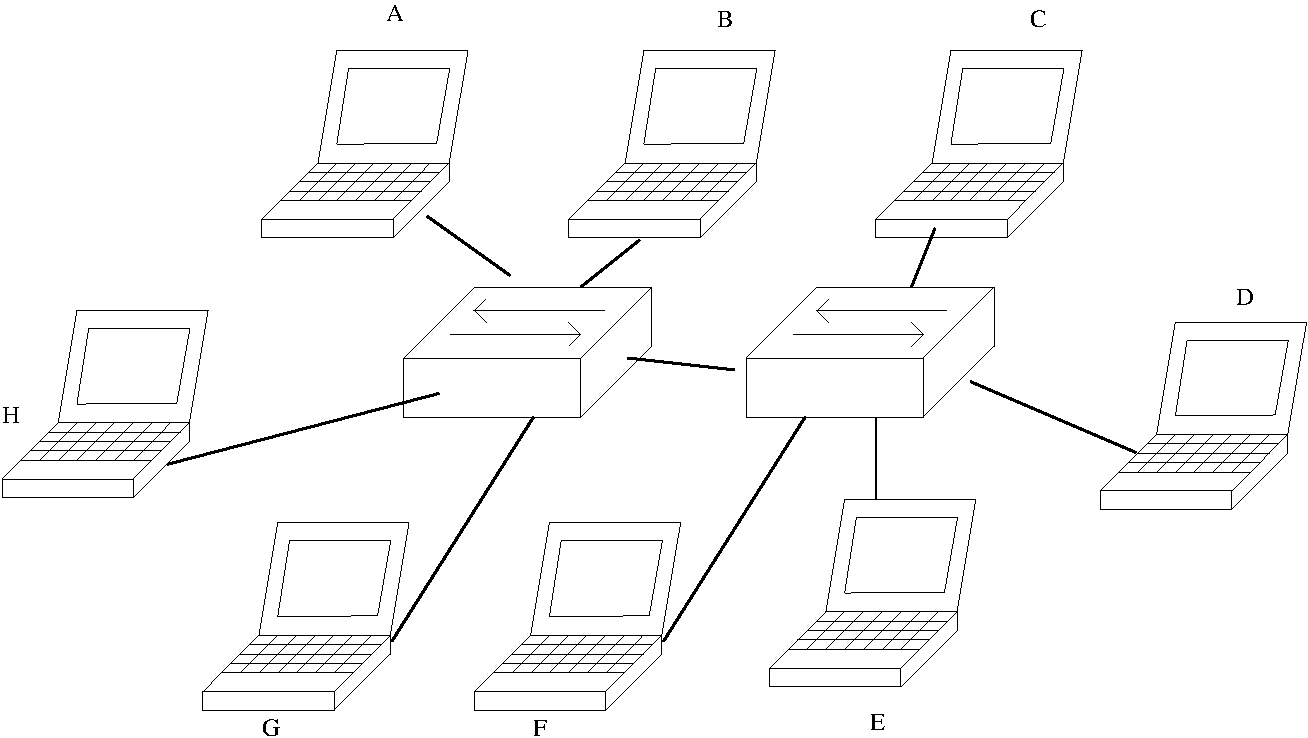
\includegraphics[width=0.5\linewidth]{Figures/No_vlan.pdf}
\else
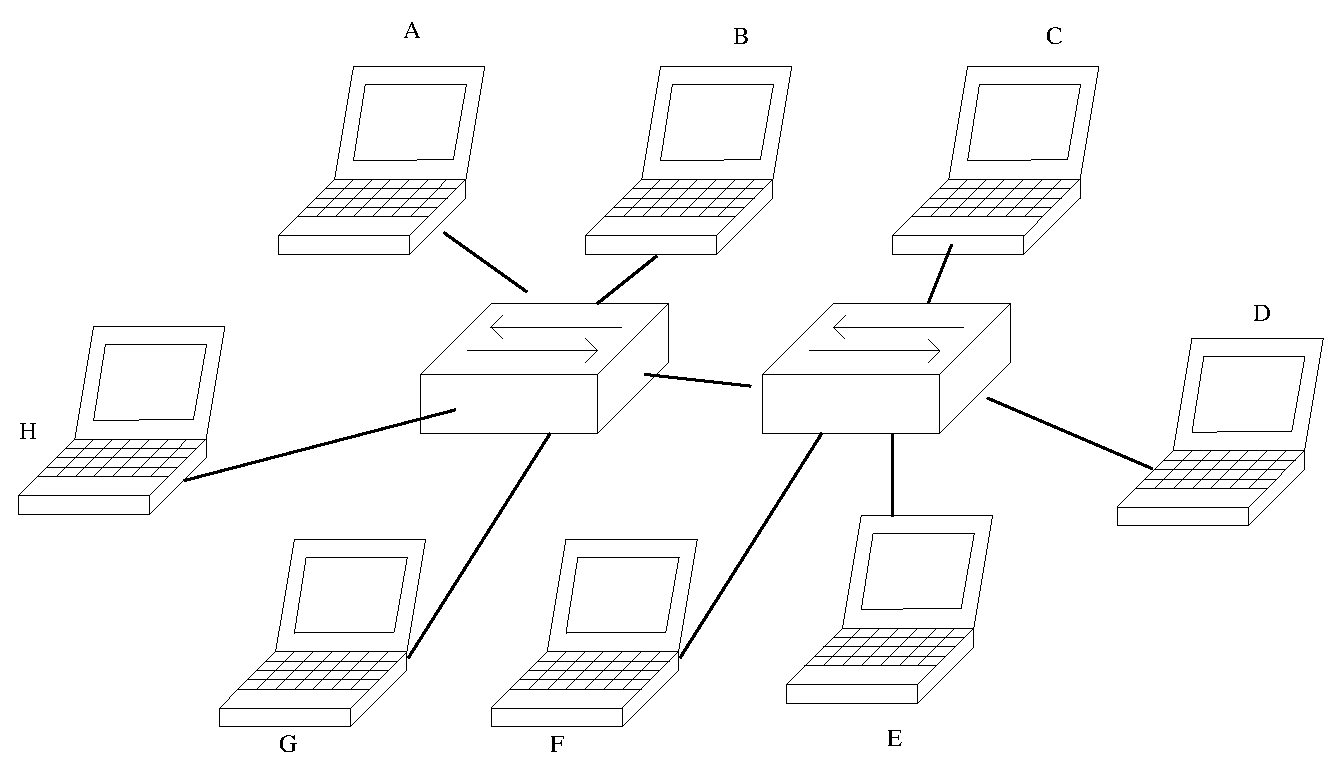
\includegraphics[width=0.5\linewidth]{Figures/No_vlan.eps}
\fi
\caption{A switched network with no VLANs.}
\label{fig:No_vlan}
\end{figure}

There are situations in which it is required to partition the network.
For example, in a campus university it might be necessary to keep wireless access points in a network separated from the servers.
If the access points are separated across multiple buildings, it would be necessary to have a switch for the access points in each building.
Similarly, if there were servers in multiple buildings, it would also be necessary to place a dedicated switch for the servers in each building.
Requiring a switch for every network in every location is a solution that does not scale as the number of locations and networks increase.
It is much more convenient to have a single switched network and then configure the switches to create virtual separate link-layer networks.
This is precisely what VLANs offer.
Fig.~\ref{fig:Vlan} shows an example with two VLANs in which computers A, B and C are kept in a link-layer network separated from D, E and F.


\begin{figure}
\centering
\ifpdf
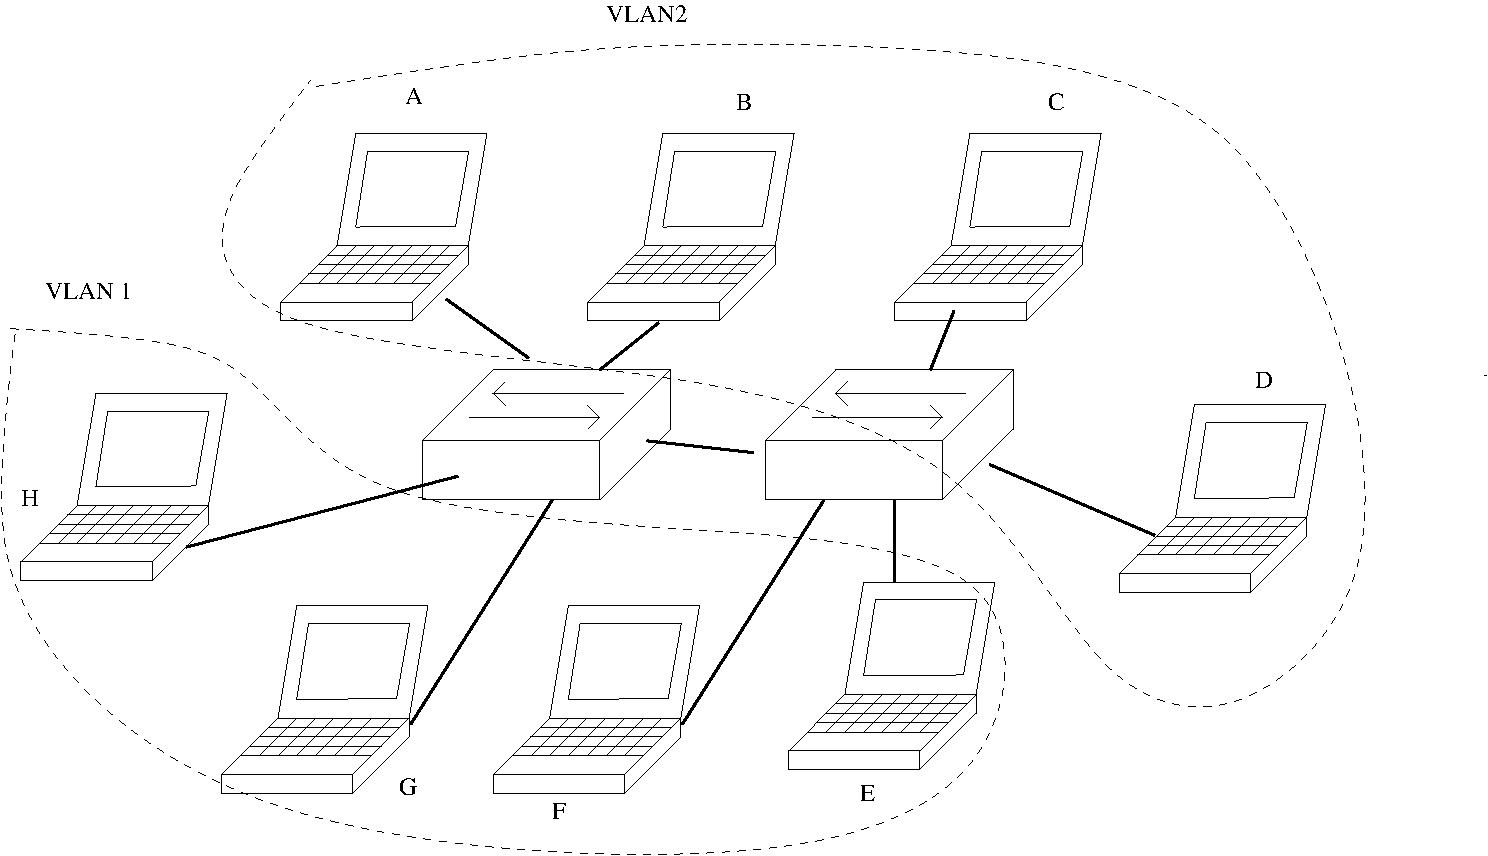
\includegraphics[width=0.5\linewidth]{Figures/Vlan.pdf}
\else
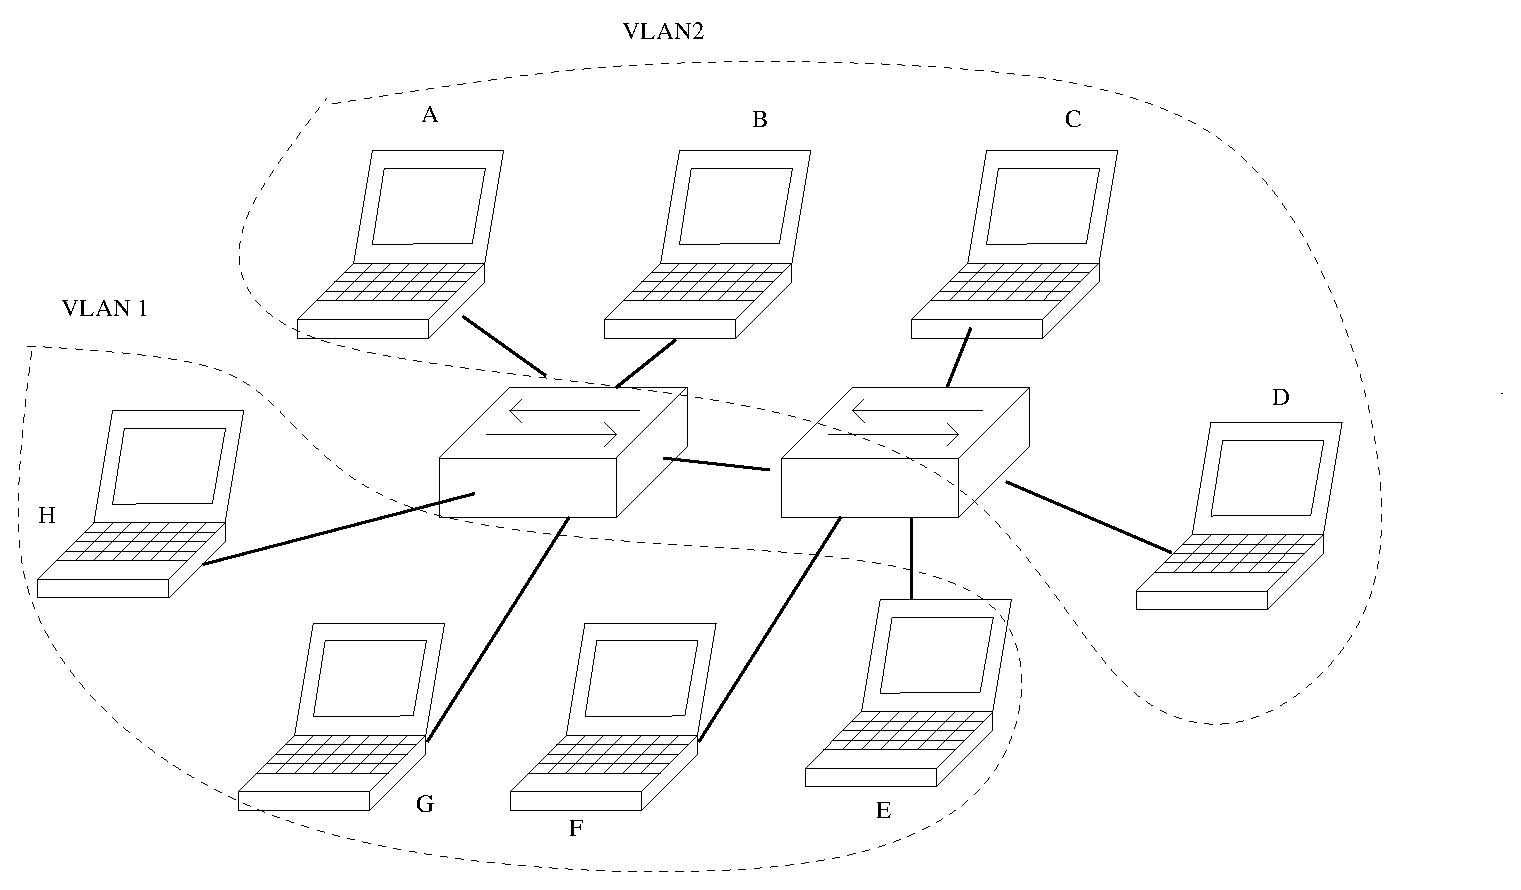
\includegraphics[width=0.5\linewidth]{Figures/Vlan.eps}
\fi
\caption{A switched network with two VLANs}
\label{fig:Vlan}
\end{figure}

VLANs are very convenient for deploying switched networks as it is possible for the network administrators to install a single switched network.
This network can later be partitioned in a flexible way simply changing the configuration of the swithches.
It is possible that ethernet ports in the same room belong to different virtual link-layer networks as it is also possible to have ethernet ports in different buildings connected to the same virtual link-layer network.

Another advantage of VLANs is that if an administrator wants to change a device from one network to another, it can simply remotely change the configuration of the switch.
It is not necessary that the technician goes to the wiring closet to physically disconnect and re-connect a cable.

\begin{figure}
\centering
\ifpdf
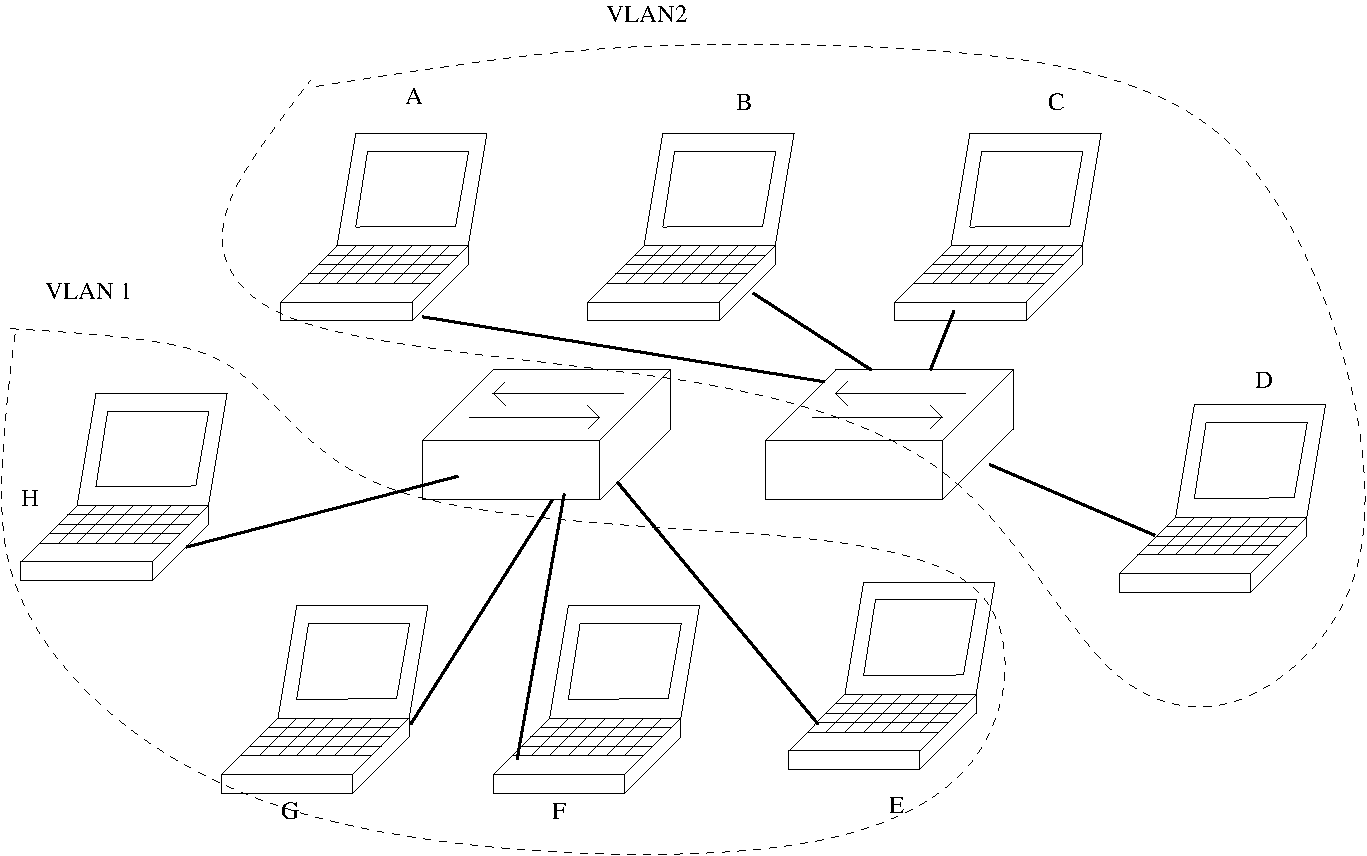
\includegraphics[width=0.5\linewidth]{Figures/Equivalent.pdf}
\else
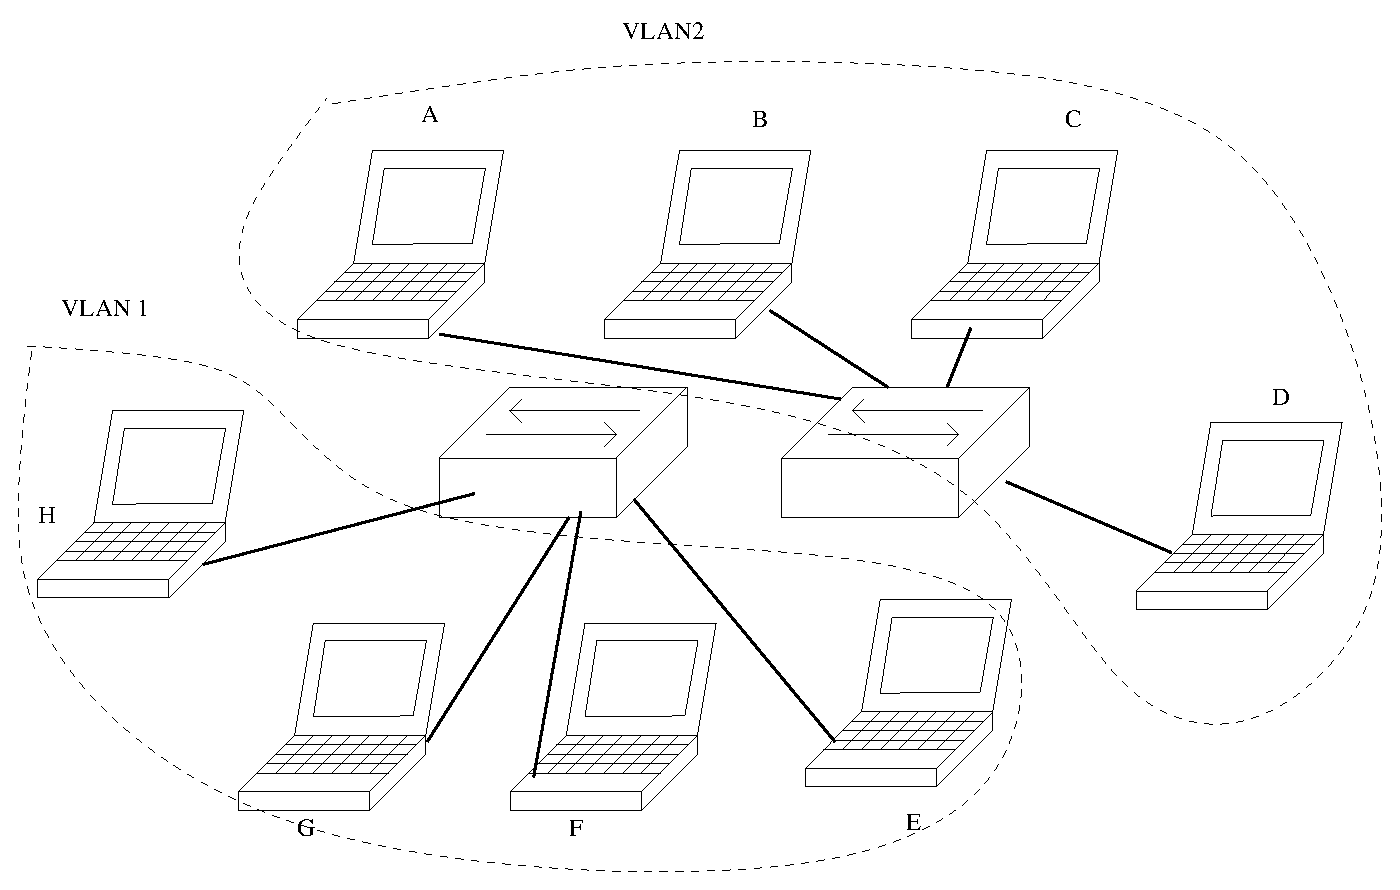
\includegraphics[width=0.5\linewidth]{Figures/Equivalent.eps}
\fi
\caption{The equivalent behaviour of the network with two VLANs depicted in Fig.~\ref{fig:Vlan}}
\label{fig:Equivalent}
\end{figure}

In a typical configuration, each VLAN contains one IP subnetwork, and it is connected to other subnetworks using a router.
Each VLAN has a number which is the VLAN identifier.
The switch ports are associated to VLAN by configuring each of the ports.  
If a switch has four ports and ports \#1 and \#3 are assigned to VLAN 10 while ports \#2 and \#4 are assigned to VLAN 20, then traffic flows from port \#1 to \#3 and the other way around, but it is isolated from ports \#2 and \#4.
This kind of assignment of a single VLAN to a port is called \emph{static-access}.


In a network deployment with multiple switches it is necessary to carry ethernet traffic from one switch to others.
One option would be to connect a separate cable for each of the existing VLANs. 
This solution is not convenient for two different reasons.
The first is that it requires many cables and many ports in each of the switches.
The second is that a new cable has to be added each time that a VLAN is created.

The alternative is to use a single cable to interconnect two routers and use that cable to transmit frames of different VLANs.
This makes the deployment and maintenance of the switched network easier.
A port carrying packets of multiple VLANs is called a trunking port.

If packets of different VLANs are transmitted over the same switch, the receiving switch needs to know to which VLAN each packet belongs to.
To this end, the sending switch will mark every frame with information about the VLAN it belongs to.
This mark is called a \emph{tag} or, more technically, IEEE 802.1Q header.

In a default configuration, switches have a default VLAN that is also the management VLAN.
Access through the management VLAN allows remote router configuration.
Extreme care should be exercised when remotely configuring VLANs to prevent cutting the management connectivity.
If this occurs, it will be necessary to physically access the switch to recover configuration.

Trunk switch ports can have a \emph{native} VLANs.
Packets that are received and not tagged are considered to belong to the native VLAN.
Similarly, frames belonging to the native VLAN are not tagged when transmitted.

Cisco devices feature a VLAN trunking protocol that propagates VLAN-related information to all the layer-2 network.
This makes it possible to see from one switch all the VLANs available in the network.


A switched network in which every device can reach any other device with level-2 connectivity is called a flat network topology.
Every broadcast packet is received by every participating device.
For performance, security or management reasons it might be a good idea to split the flat topology in two or more VLANs.

Each VLAN is a single broadcast domain.
A broadcast packet by a host connected to a particular VLAN will reach all the devices connected to that VLAN.
Importantly, that broadcast packet will not reach devices that are not connected to the same VLAN as the sender.

Two devices connected to the same VLAN have layer-2 connectivity and can directly exchange packets without requiring the intervention of a router.
Devices connected to different VLANs need a router or layer-3 switch to exchange packets.

Another terminology used to refer to VLANs is \emph{logical network segment} as opposed to a \emph{physical network segment}.
The former is created using configuration while the latter consists of actual physical cables.

The VLANs are created by assigning the ports of the switch to a given VLAN. 
There are two ways of making this assignment: static and dynamic. 

\subsection{Static Assignment}

In the static assignment the network administrator assign a particular port to a particular VLAN.
The end host connected to that port will see other hosts connected to that VLAN and it doesn't need to be aware that there is a VLAN.
A switch can have ports in different VLANs and VLANs can have ports in multiple switches.

By default all ports on a switch are connected to VLAN 1.
To change a port to another VLAN, it is necessary to first create the other VLAN if it does not exist.

\begin{lstlisting}
Switch(config)# vlan vlan-num
Switch(config-vlan)# vlan vlan-name
\end{lstlisting}

The assignment of a name to the VLAN is optional. 
The name, if given, must not contain blank spaces.

For example, to create VLANs for the classrooms and for the WiFi access points we use:

\begin{lstlisting}
Switch(config)# vlan 3
Switch(config-vlan)# vlan classrooms
Switch(config)# vlan 12
Switch(config-vlan)# vlan wifi-access-point
\end{lstlisting}

A VLAN can be deleted issuing the \texttt{no vlan vlan-num} command.

After creating a VLAN, the ports of the switch can be assigned to that VLAN.
The commands are:
\begin{lstlisting}
Switch(config)# interface type module/number
Switch(config-if)# switchport
Switch(config-if)# switchport mode access
Switch(config-if)# switchport access vlan vlan-num
\end{lstlisting}

The \texttt{switchport mode access} command configures the port as an access port, which is typically used to connect a host.
Then, the \texttt{ switchport access vlan vlan-num} assignst that port to a particular VLAN.
This port will belong to a single VLAN and the host attached to that port will belong to that VLAN.

The commands \texttt{show vlans} and \texttt{show vlans brief} can be used to display VLAN port assignment information.

\begin{lstlisting}
user@switch> show vlans

Name           Tag     Interfaces
default        None
                       ge-0/0/34.0, ge-0/0/33.0, ge-0/0/32.0, ge-0/0/31.0,
                       ge-0/0/30.0, ge-0/0/29.0, ge-0/0/28.0, ge-0/0/27.0,
                       ge-0/0/26.0, ge-0/0/25.0, ge-0/0/19.0, ge-0/0/18.0,
                       ge-0/0/17.0, ge-0/0/16.0, ge-0/0/15.0, ge-0/0/14.0,
                       ge-0/0/13.0, ge-0/0/11.0, ge-0/0/9.0, ge-0/0/8.0,
                       ge-0/0/3.0, ge-0/0/2.0, ge-0/0/1.0
v0001          1
                       ge-0/0/24.0, ge-0/0/23.0, ge-0/0/22.0, ge-0/0/21.0
v0002          2
                       None
v0003          3
                       None
v0004          4
                       None
v0005          5
                       None

user@switch> show vlans brief

                                           Ports
Name           Tag     Address             Active/Total
default        None                        0/23
v0001          1                           0/4
v0002          2                           0/0
v0003          3                           0/0
v0004          4                           0/0
v0005          5                           0/0
v0006          6                           0/0
v0007          7                           0/0
v0008          8                           0/0
v0009          9                           0/0
v0010          10                          0/2
v0011          11                          0/0
v0012          12                          0/0
v0013          13                          0/0
v0014          14                          0/0
v0015          15                          0/0
v0016          16                          0/0

\end{lstlisting}

\section{Dynamic Assignment}

The dynamic assignment of ports to VLANs requires to create an association between end devices MAC addresses and VLANs.
Then, when an end device is connected to a switch, the switch queries a database to find out the VLAN to which the MAC address of the connected device belongs.
Then the switch dynamically configures that VLAN to the port.

The advantage is that a user can connect to different ports and always be in the same VLAN.
This can be useful for example for a person working in different offices or buildings.

\section{Trunking}

End devices typically connected to switch ports that belong to a single VLAN, and the host does not need to know anything about the VLAN.
The situation is different in connections between two switches.
When two switches need to exchange traffic of two or more VLANs it can be a good idea to connect them using trunking ports.
Trunking are also useful to connect switches to routers.

A trunking port carries traffic of different VLANs.
The receiving end needs to know to which VLAN each frame belongs to.
For this purpose, the sender marks sent packets including a VLAN ID field in the packet headers.
This information is also called a tag.
The receiver uses the tag to know tho which VLAN the packet belongs to and removes the tag.
The tag will be added again if the receiving end needs to re-transmit the packet over another trunk connection.
If a frame is sent to a host device over an access port, the tag is not included and therefore the host does not have any information regarding the VLAN ID.

The Catalyst switches that we use in this course have two different mechanisms to attach a tag to the frames.
The first one is using Cisco's proprietary Inter-Switch Link (ISL) protocol.
The second is using the standard IEEE 802.1Q protocol.

IEEE 802.1Q protocol inserts a 4-byte tag between the source address field and the frame length field in the layer-2 header.
The first two bytes are the Tag Protocol Identifier (TPID) and are always set to 0x8100 to indicate that it is a 802.1Q tag.
Of the remaining 16 bits, 3 of them are the priority field, 1 is the Canonical Format Indicator (CFI) and the other 12 are the VLAN ID.

Cisco switches implement a proprietary Dynamic Trunking Protocol that allow two networking devices to negotiate the trunk status of a link between the two of them.
It is also possible to statically configure a port as a trunking port.

The commands to configure a port as trunk are:

\begin{lstlisting}
Switch(config)# interface type mod/port
Switch(config-if)# switchport
Switch(config-if)# switchport trunk encapsulation {isl | dot1q | negotiate}
Switch(config-if)# switchport trunk native vlan vlan-id
Switch(config-if)# switchport trunk allowed vlan {vlan-list | all |
{add | except | remove} vlan-list}
Switch(config-if)# switchport mode {trunk | dynamic {desirable | auto}}
\end{lstlisting}

The encapsulation decides which of the possible alternatives to tag the frames will be used.
In the case of a IEEE 802.1Q, it is necessary to configure a native vlan.
This vlan will be transmitted without a tag.
The same native vlan needs to be configured at both ends of the connection.

Then it is possible to configure which VLANs will be transmitted over this trunk.
This configuration should be the same in both ends of the link.

And finally, there is the option to configure the mode as trunk or dynamic.
In the case of trunk, the port will always be a trunk.
In the case of dynamic desirable, the port will try to convince the other end to establish a trunk.
Finally, in the case of dynamic auto, the port will switch to trunk only if the other end asks so.

The command \texttt{show interfaces trunk} provides information about trunking.
\begin{lstlisting}
Cat3550#show interfaces trunk 

Port      Mode         Encapsulation  Status        Native vlan
Fa0/17  trunk    802.1q         trunking   1
Fa0/18  trunk    802.1q         other      1
Fa0/19  trunk    802.1q         other      1

Port      Vlans allowed on trunk Fa0/17     1-4094 Fa0/18     1-4094
Fa0/19     1-4094

Port      Vlans allowed and active in management domain Fa0/17     1-3,10 
Fa0/18     1-3,10
Fa0/19     None

Port      Vlans in spanning tree forwarding state and not pruned  
Fa0/17    1-3,10

Fa0/18    1-3,10

Fa0/19    None
\end{lstlisting}

